\subsection{Generowanie ruchów pseudolegalnych}
\label{subsec:generowanie-ruchow-pseudolegalnych}

\subsubsection{Generowanie ruchów piona}

Pionek na szachownicy ma do dyspozycji parę możliwych ruchów, które zależą od aktualnej pozycji na planszy: ruch o pole do przodu, początkowy ruch o dwa pola do przodu, bicie na skos w lewo bądź prawo, bicie en-passant.
Powyższe ruchy zostały zaimplementowane przez operacje bitowe i bitowe przesunięcia na masce bitowej reprezentującej pionki.
Dla przykładu technika generowania ruchów piona o jedno pole do przodu:

\begin{figure}[ht]
    \centering
    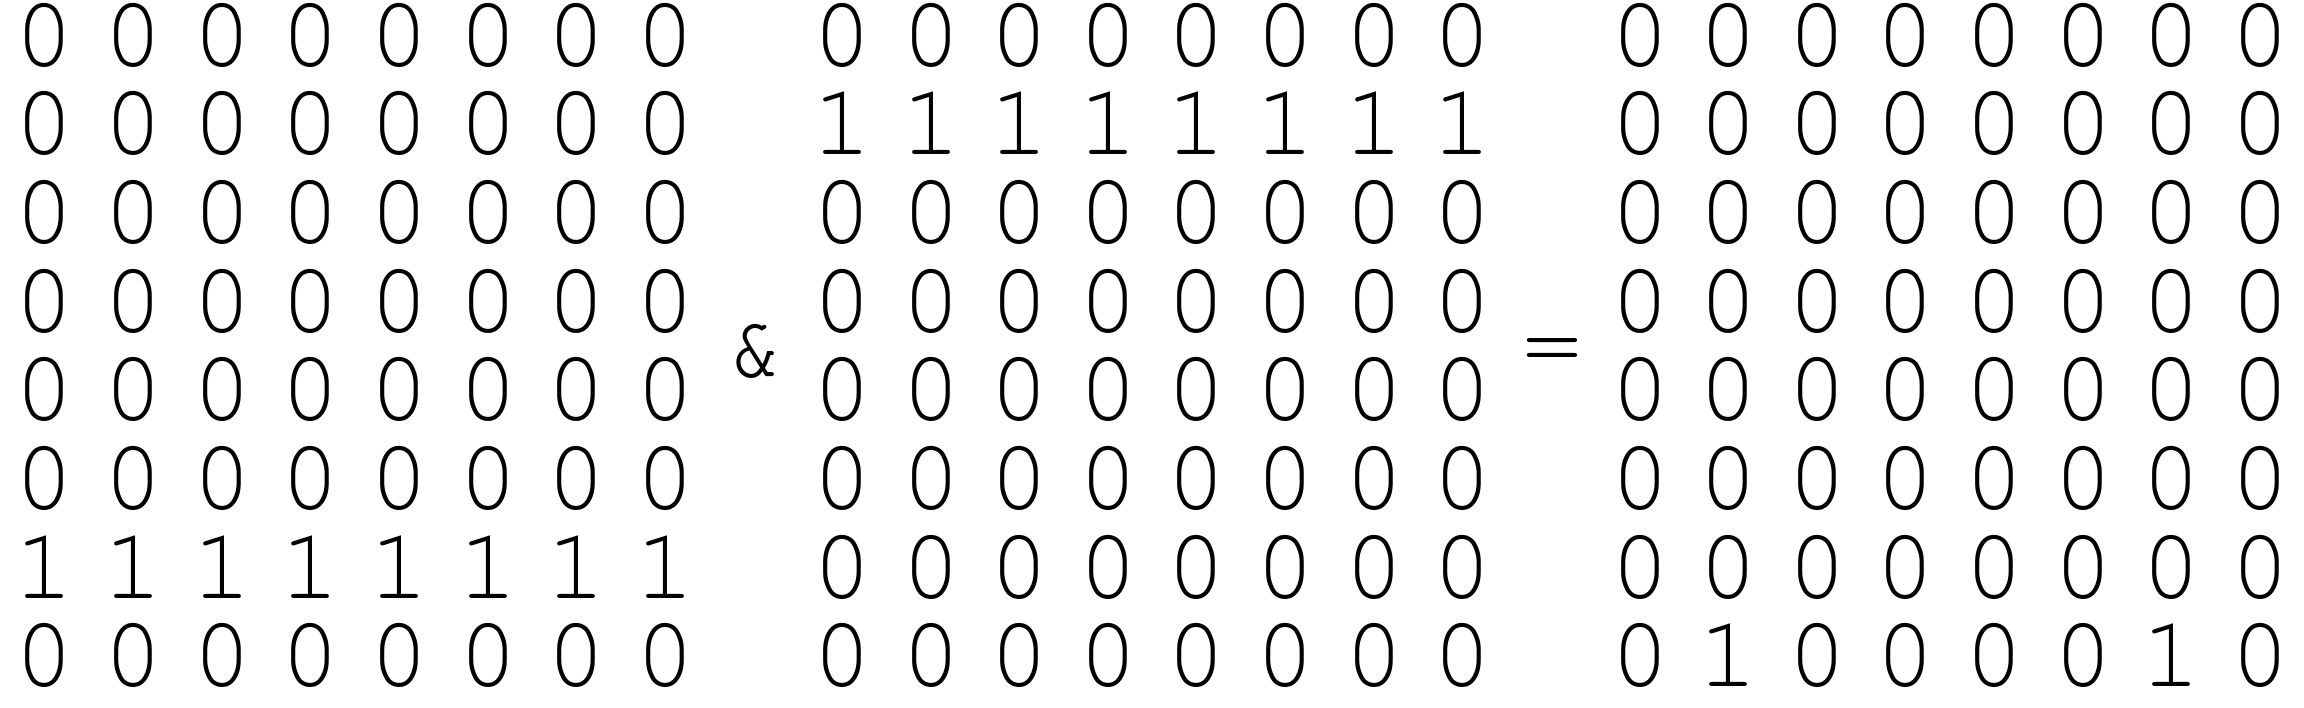
\includegraphics[width=0.85\linewidth]{rozdzialy/rozdzial01/3_generowanie-ruchow/rysunki/bitboards-arithmetic}
    \caption{Kodowanie ruchu szachowego}
    \label{fig:bitboards-arithmetic}
\end{figure}


\subsubsection{Generowanie ruchów hetmana, wieży i gońca}

\subsubsection{Generowanie ruchów króla i skoczka}

